\documentclass[a4paper,notitlepage]{article}

\usepackage{xltxtra}
\usepackage{amsmath}
\usepackage{amssymb}
\usepackage{amsthm}
\usepackage{tikz}
\usepackage{unicode-math}
\usepackage{fontspec}
\usepackage{multicol}
\usepackage{faktor}
\usetikzlibrary{positioning}
\setmathfont{xits-math.otf}

\newtheorem{definition}{Definition}
\newtheorem{proposition}{Proposition}


\tikzset{node distance=2cm, auto}

\author{Víctor López Juan}
\title{Chapter 5}

\begin{document}
\maketitle
\begin{enumerate}

  \item[8.]

    \begin{proposition}
      
    For a category {\bf C}, define the objects of $\text{\bf Par}(\text{\bf C})$
    as those of {\bf C}, and an arrow $f : A → B$ as a pair $(\vert f \vert, U_f)$,
    where $U_f$ is a subobject of $A$,  $\vert f \vert : U_f → B$.

    Composition is defined by taking a pullback and then composing:

           
           \begin{tikzpicture}

             \node (A) {$A$};
             \node (Uf) [above of=A] {$U_f$};

             \node (B) [right of=Uf] {$B$};
             \node (Ug) [above of=B] {$U_g$};

             \node (Ug2) [above of=Uf] {$\vert f \vert ^\star (U_{g})$};

             \node (C) [right of=Ug] {$C$};

             \draw [>->] (Uf) to node {$m_1$} (A);
             \draw [>->] (Ug) to node {$m_2$} (B);

             \draw [->]  (Uf) to node {$\vert f \vert$} (B);
             \draw [->]  (Ug) to node {$\vert g \vert$} (C);
             


             \draw [>->] (Ug2) to node {$m_2^\prime$} (Uf);
             \draw [->]  (Ug2) to node {$\bar{\vert f \vert}$} (Ug);
          \end{tikzpicture}


    The composition of two arrows is in $\text{\bf Par}(\text{\bf C})$, and
    $\text{\bf Par}(\text{\bf C})$ is a category.

    \end{proposition}

    \begin{proof}
    \begin{itemize}
      \item

        
        First, observe that:
        
      \begin{itemize}
        \item The arrow $\vert f \vert^\star (U_g) \rightarrowtail U_f$
          is monic, because the diagram is a pullback.

        \item $\vert f \vert ^\star (U_g)$ is a subobject of A.

      \end{itemize}

        Therefore, composition is well-defined, as it produces an arrow
        in the category.

      \item There must be identity arrows for every object.

        \begin{itemize}
          \item For every object, there is an identity arrow:

            \begin{tikzpicture}
              \node (A) {$A$};
              \node (A2) [right of=A] {$A$};
              \node (A3) [below of=A] {$A$};
    
              \draw [->] (A) to node {$id_A$} (A2);
              \draw [>->] (A) to node {$id_A$} (A3);
            \end{tikzpicture}
    
            It can be both left and right composed with other arrows:

            \begin{multicols}{2}
              
            \begin{tikzpicture}
              \node (A) {$A$};
              \node (A2) [right of=A] {$A$};
              \node (A3) [below of=A] {$A$};

              \node (Uf) [above of=A2] {$U_f$};
              \node (Uf2) [above of=A] {$U_f$};
              \node (B)  [right of=Uf] {$B$};
              
    
              \draw [->] (A) to node {$id_A$} (A2);
              \draw [>->] (A) to node {$id_A$} (A3);
              \draw [>->] (Uf) to node {$m$} (A2);
              \draw [>->] (Uf2) to node {$m$} (A);
              \draw [->] (Uf) to node {$\vert f \vert$} (B);
              \draw [->] (Uf2) to node {$id_{U_f}$} (Uf);
            \end{tikzpicture}


            \begin{tikzpicture}

              \node (Uf) {$U_f$};
              \node (A)  [below of=Uf] {$A$};
              \node (Uf2) [above of=Uf] {$U_f$};
              
              \node (B)  [right of=Uf] {$B$};
              \node (B2) [above of=B] {$B$};
              \node (B3) [right of=B2] {$B$};

    
              \draw [->] (B2) to node {$id_B$} (B3);
              \draw [>->] (B2) to node {$id_B$} (B);
              \draw [>->] (Uf) to node {$m$} (A);
              \draw [->] (Uf) to node {$\vert f \vert$} (B);
              \draw [->] (Uf2) to node {$\vert f \vert$} (B2);
              \draw [>->] (Uf2) to node {$id_{U_f}$} (Uf);
            \end{tikzpicture}

            \end{multicols}
              
            In both cases, the pullback of the diagram is the object
            $U_f$ itself; it is universal with this property.

            \begin{multicols}{2}
              
            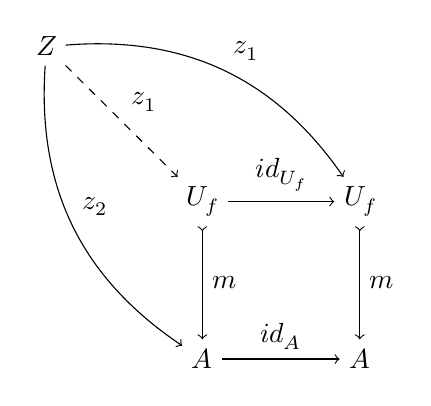
\begin{tikzpicture}
              \node (A) {$A$};
              \node (A2) [right of=A] {$A$};

              \node (Uf) [above of=A2] {$U_f$};
              \node (Uf2) [above of=A] {$U_f$};
              
              \node (Z) [above left=of Uf2] {$Z$};
    
              \draw [->] (A) to node {$id_A$} (A2);
              \draw [>->] (Uf) to node {$m$} (A2);
              \draw [>->] (Uf2) to node {$m$} (A);
              \draw [->] (Uf2) to node {$id_{U_f}$} (Uf);
              
              \draw [->,bend left] (Z) to node {$z_1$} (Uf);
              \draw [->,bend right] (Z) to node {$z_2$} (A);
              \draw [->,dashed] (Z) to node {$z_1$} (Uf2);
            \end{tikzpicture}


            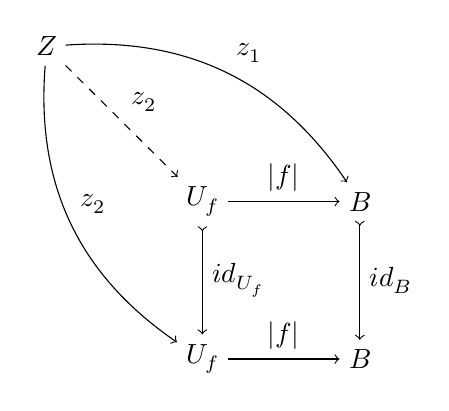
\begin{tikzpicture}
              \node (Uf) {$U_f$};
              \node (B)  [right of=Uf] {$B$};
              \node (Uf2) [above of=Uf] {$U_f$};
              \node (B2) [above of=B] {$B$};

              \node (Z) [above left=of Uf2] {$Z$};

              \draw [>->] (B2) to node {$id_B$} (B);
              \draw [->] (Uf) to node {$\vert f \vert$} (B);
              \draw [->] (Uf2) to node {$\vert f \vert$} (B2);
              \draw [>->] (Uf2) to node {$id_{U_f}$} (Uf);

              \draw [->,bend left] (Z) to node {$z_1$} (B2);
              \draw [->,bend right] (Z) to node {$z_2$} (Uf);
              \draw [->,dashed] (Z) to node {$z_2$} (Uf2);
            \end{tikzpicture}

            \end{multicols}

            Therefore, identity arrows are both the right and left
            identity for composition.

        \item Composition is associative.

           
           \begin{tikzpicture}

             \node (A) {$A$};
             \node (Uf) [above of=A] {$U_f$};

             \node (B) [right of=Uf] {$B$};
             \node (Ug) [above of=B] {$U_g$};

             \node (C) [right of=Ug] {$C$};
             \node (Uh) [above of=C] {$U_h$};

             \node (D) [right of=Uh] {$D$};

             \draw [>->] (Uf) to node {$m_1$} (A);
             \draw [>->] (Ug) to node {$m_2$} (B);
             \draw [>->] (Uh) to node {$m_3$} (C);

             \draw [->]  (Uf) to node {$\vert f \vert$} (B);
             \draw [->]  (Ug) to node {$\vert g \vert$} (C);
             \draw [->]  (Uh) to node {$\vert h \vert$} (D);
          \end{tikzpicture}


          The composition can be computed either as $(f \circ g) \circ
          h$, or $f \circ (g \circ h)$.

          \begin{multicols}{2}

          {\small
          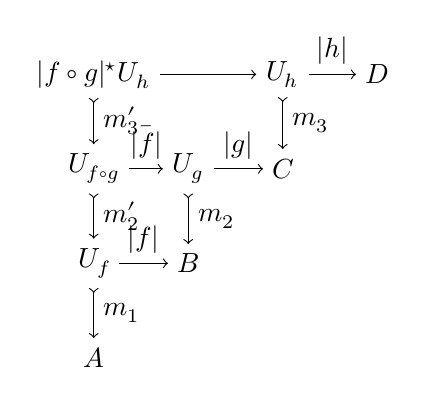
\begin{tikzpicture}[node distance=1.2cm]

             \node (A) {$A$};
             \node (Uf) [above of=A] {$U_f$};

             \node (B) [right of=Uf] {$B$};
             \node (Ug) [above of=B] {$U_g$};
             \node (Ug2) [above of=Uf] {$U_{f \circ g}$};

             \node (C) [right of=Ug] {$C$};
             \node (Uh) [above of=C] {$U_h$};
             
             \node (Uh2) [above of=Ug2] {$\vert f \circ g \vert^\star U_h$};

             \node (D) [right of=Uh] {$D$};

             \draw [>->] (Uf) to node {$m_1$} (A);
             \draw [>->] (Ug) to node {$m_2$} (B);
             \draw [>->] (Ug2) to node {$m_2^\prime$} (Uf);
             \draw [>->] (Uh) to node {$m_3$} (C);

             \draw [->]  (Ug2) to node {$\bar{\vert f \vert}$} (Ug);
             
             \draw [->]  (Uf) to node {$\vert f \vert$} (B);
             \draw [->]  (Ug) to node {$\vert g \vert$} (C);
             \draw [->]  (Uh) to node {$\vert h \vert$} (D);

             \draw [>->] (Uh2) to node {$m_3^\prime$} (Ug2);
             \draw [->] (Uh2) to node {} (Uh);
          \end{tikzpicture}

         
           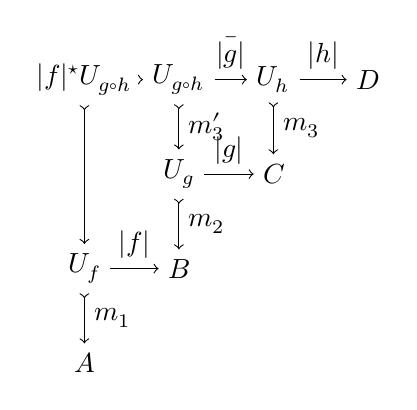
\begin{tikzpicture}[node distance=1.2cm]

             \node (A) {$A$};
             \node (Uf) [above of=A] {$U_f$};

             \node (B) [right of=Uf] {$B$};
             \node (Ug) [above of=B] {$U_g$};

             \node (C) [right of=Ug] {$C$};
             \node (Uh) [above of=C] {$U_h$};

             \node (Uh2) [above of=Ug] {$U_{g \circ h}$};
             
             \node (Ug2) [left of=Uh2] {$\vert f \vert^\star U_{g \circ h}$};

             \node (D) [right of=Uh] {$D$};

             \draw [>->] (Uf) to node {$m_1$} (A);
             \draw [>->] (Ug) to node {$m_2$} (B);
             \draw [>->] (Uh) to node {$m_3$} (C);

             \draw [>->] (Uh2) to node {$m_3^\prime$} (Ug);
             
             \draw [>->] (Ug2) to node {} (Uf);
             
             \draw [->]  (Uf) to node {$\vert f \vert$} (B);
             \draw [->]  (Ug) to node {$\vert g \vert$} (C);
             \draw [->]  (Uh) to node {$\vert h \vert$} (D);

             \draw [->]  (Uh2) to node {$\bar{\vert g \vert}$} (Uh);


             \draw [->]  (Ug2) to node {} (Uh2);
             
          \end{tikzpicture}
           }

           \end{multicols}

           To prove that they are equivalent, we use a hybrid approach
           to construct a third composition arrow, $U_{(f \circ g) \circ h}$.

           \begin{tikzpicture}

             \node (A) {$A$};
             \node (Uf) [above of=A] {$U_f$};

             \node (B) [right of=Uf] {$B$};
             \node (Ug) [above of=B] {$U_g$};

             \node (C) [right of=Ug] {$C$};
             \node (Uh) [above of=C] {$U_h$};

             \node (Ugh) [above of=Ug] {$U_{g \circ h}$};
             \node (Ufg) [above of=Uf] {$U_{f \circ g}$};
             
             \node (Ufgh) [above of=Ufg] {$U_{f \circ g \circ h}$};


             \draw [->]  (Ufg) to node {$\bar{\vert f \vert}$} (Ug);
             \draw [->]  (Ugh) to node {$\bar{\vert g \vert}$} (Uh);
             \draw [->]  (Ufgh) to node {} (Ugh);

             \node (D) [right of=Uh] {$D$};

             \draw [>->] (Uf) to node {$m_1$} (A);
             \draw [>->] (Ug) to node {$m_2$} (B);
             \draw [>->] (Uh) to node {$m_3$} (C);

             \draw [>->] (Ufg) to node {} (Uf);
             \draw [>->] (Ugh) to node {} (Ug);
             \draw [>->] (Ufgh) to node {} (Ufg);

             \draw [->]  (Uf) to node {$\vert f \vert$} (B);
             \draw [->]  (Ug) to node {$\vert g \vert$} (C);
             \draw [->]  (Uh) to node {$\vert h \vert$} (D);
          \end{tikzpicture}


          By the two pullback lemma, two pullback squares can be joined
          together to form a pullback of the outer rectangle.

          Because pullbacks are unique up to isomorphism, applying the
          lemma to either the horizontal or the vertical rectangle
          in the diagram yields, respectively, the isomorphisms:

          
          $$ U_{f \circ g \circ h} \cong \vert f \circ g \vert^\star (U_h)$$

          $$ U_{f \circ g \circ h} \cong \vert f \vert^\star U_{g\circ h} $$

        \end{itemize}
        
   \end{itemize}

   \end{proof}

   \item[13.]

     Consider the sequences:

     $$ M_0 → M_1 → M_2 → … \, , \, g_i : M_i → M_{i+1} $$
     $$ N_0 ← N_1 ← N_2 ← … \, , \, g_i : N_{i+1} → N_{i} $$
     
     
     For every chain of homomorphisms,  $\left\{g_i\right\}_{i=1}^\infty$, define:
     $$g_{i,k} = g_{k-1} \circ … \circ g_{i+1} \circ g_i$$

     In particular, $g_{i,i} = id_{cod(g_i)}$.


     We are interested in the limits and colimits of these sequences.

     Limits in {\bf Mon} can be defined in terms of (co)products and (co)equalizers
     in {\bf Set}. If this constructions have adequate properties, they
     can be given a monoid structure, which gives existence in {\bf Mon}.

     Uniqueness in {\bf Set} is derived by factoring uniquely
     over (co)products and (co)equalizers, which are themselves universal.

     For example:

     \begin{itemize}
       \item
         
         $$M = \lim_{\longrightarrow} M_i = \faktor{\coprod M_i}{\sim}$$

         Where $\sim$ is defined as the equivalence relation that makes
         the following diagram commutes for every $i \in \mathbb{N}$. 

         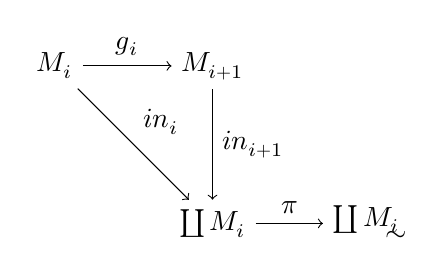
\begin{tikzpicture}
           \node (Mi) {$M_i$};
           \node (Mip) [right of=Mi] {$M_{i+1}$};
           \node (Cop) [below of=Mip] {$\coprod M_i$};
           \node (Q) [right of=Cop] {$\faktor{\coprod M_i}{\sim}$};

           \draw[->] (Cop) to node {$\pi$} (Q);
           \draw[->] (Mi) to node {$g_i$} (Mip);
           \draw[->] (Mi) to node {$in_{i}$} (Cop);
           \draw[->] (Mip) to node {$in_{i+1}$} (Cop);
         \end{tikzpicture}

         
         Then, $(M, \star, 1_M)$ is a monoid, where:

         \begin{itemize}
           
           \item Identity is the projection of any of the identity
             elements of the monoids in the chain.
             
         $$\forall i,\,1_M = \left [ 1_{i} \right ]$$
           \item  
         For elements $[x]$, $[y]$ in $M$, $x \in M_i$, $y \in M_j$; let
         $(M_k, \star_k)$ be a monoid such that $k \geq i,j$.

         $$[x] \star [y] = \left [ g_{i,k}(x) \star_k g_{j,k}(y) \right ]$$

         The definition is independent of the choice of $k$, and the
         choice of representatives, due to the commutativity of the
         diagrams above.

         \end{itemize}
         
         The arrows $\pi \circ in_i : M_i → M$ are monoid homomorphisms.

         $M$ is universal for the property of having arrows from every
         element in the chain to itself, as shown by the following diagram:
 
         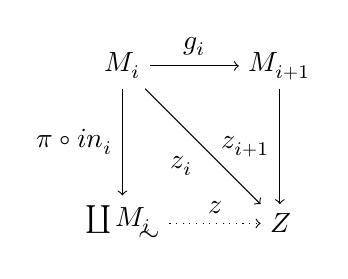
\begin{tikzpicture}

           \node (Mi) {$M_i$};
           \node (Q) [below of=Mi] {$\faktor{\coprod M_i}{\sim}$};
           \node (Mip) [right of=Mi] {$M_{i+1}$};
           \node (Z)  [right of=Q] {$Z$};

           \draw[->] (Mi) to node {$g_{i}$} (Mip);
           \draw[->] (Mi) to node [left] {$\pi \circ in_i$} (Q);
           \draw[->,dotted] (Q) to node {$z$} (Z);
           \draw[<-] (Z) to node {$z_i$} (Mi);
           \draw[<-,left] (Z) to node {$z_{i+1}$} (Mip);

         \end{tikzpicture}

         $$z = \left [ z_0, z_1, …, \right ]  $$

         Uniqueness of $z$ is derived from the universality of the
         underlying construction in {\bf Set}.

         Therefore, $M$ is the colimit monoid.

       \item
         
         $$\lim_{\longleftarrow} M_i \cong M_0$$

         Instead of constructing the limit in {\bf Set}, we
         can realize that first element of the chain could be a limit.
         
         $M_0$ is a monoid, and is universal; as shown by the following
         family of diagrams:

         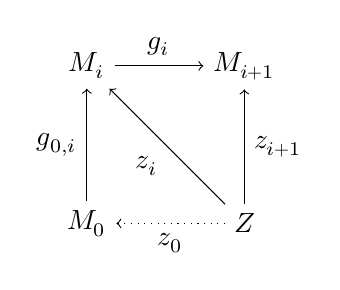
\begin{tikzpicture}

           \node (Mi) {$M_i$};
           \node (M0) [below of=Mi] {$M_0$};
           \node (Mip) [right of=Mi] {$M_{i+1}$};
           \node (Z)  [right of=M0] {$Z$};

           \draw[->] (Mi) to node {$g_{i}$} (Mip);
           \draw[->] (M0) to node {$g_{0,i}$} (Mi);
           \draw[->,dotted] (Z) to node {$z_0$} (M0);
           \draw[->] (Z) to node {$z_i$} (Mi);
           \draw[->] (Z) to node[right] {$z_{i+1}$} (Mip);
           
         \end{tikzpicture}

         In particular, for $i=0$, the arrow is unique:

         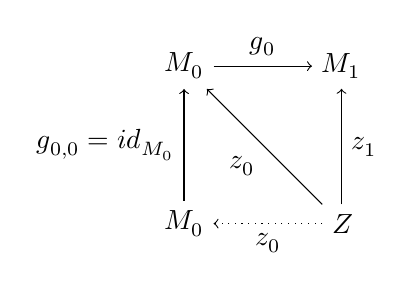
\begin{tikzpicture}

           \node (Mi) {$M_0$};
           \node (M0) [below of=Mi] {$M_0$};
           \node (Mip) [right of=Mi] {$M_{1}$};
           \node (Z)  [right of=M0] {$Z$};

           \draw[->] (Mi) to node {$g_{0}$} (Mip);
           \draw[->] (M0) to node {$g_{0,0} = id_{M_0}$} (Mi);
           \draw[->,dotted] (Z) to node {$z_0$} (M0);
           \draw[->] (Z) to node {$z_0$} (Mi);
           \draw[->] (Z) to node[right] {$z_{1}$} (Mip);
           
         \end{tikzpicture}

       \item

        
         $$N_0 = \lim_{\longrightarrow} N_i$$ 

         The colimit of this chain is its first element. Its
         universality is shown by this family of diagrams.

          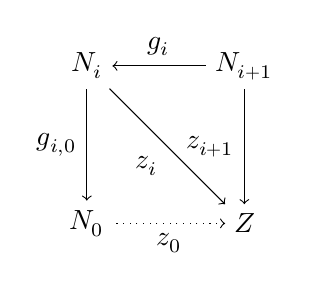
\begin{tikzpicture}

           \node (N0) {$N_{i}$};
           \node (N0p) [below of=N0] {$N_0$};
           \node (Ni) [right of=N0] {$N_{i+1}$};
           \node (Z)  [right of=N0p] {$Z$};

           \draw[<-] (N0p) to node {$g_{i,0}$} (N0);
           \draw[<-,dotted] (Z) to node {$z_0$} (N0p);
           \draw[<-] (Z) to node {$z_i$} (N0);
           \draw[<-] (Z) to node {$z_{i+1}$} (Ni);
           \draw[<-] (N0) to node {$g_i$} (Ni);
           
         \end{tikzpicture}

          Uniqueness of $z_0$ can be seen when $i = 0$.
          
          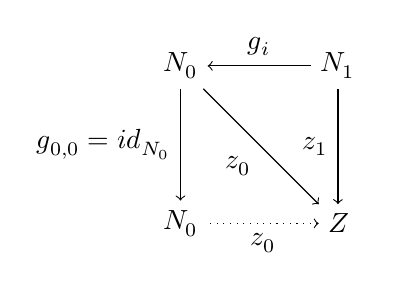
\begin{tikzpicture}

           \node (N0) {$N_{0}$};
           \node (N0p) [below of=N0] {$N_0$};
           \node (Ni) [right of=N0] {$N_{1}$};
           \node (Z)  [right of=N0p] {$Z$};

           \draw[<-] (N0p) to node {$g_{0,0} = id_{N_0}$} (N0);
           \draw[<-,dotted] (Z) to node {$z_0$} (N0p);
           \draw[<-] (Z) to node {$z_0$} (N0);
           \draw[<-] (Z) to node {$z_{1}$} (Ni);
           \draw[<-] (N0) to node {$g_i$} (Ni);
           
         \end{tikzpicture}


       \item  

         $$N = \lim_{\longleftarrow} N_i = \left . {\prod N_i} \right \vert _P$$

         … where $P$ is a predicate such that the following family of
         diagrams in {\bf Set} commutes, $i \in \mathbb{N}$.

         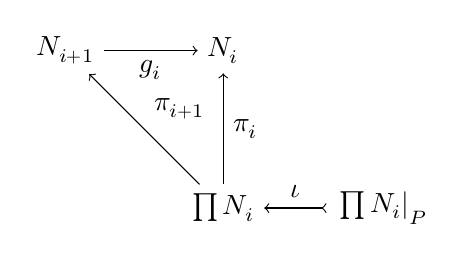
\begin{tikzpicture}
           \node (Ni) {$N_i$};
           \node (Nip) [left of=Ni] {$N_{i+1}$};
           \node (Prod) [below of=Ni] {$\prod N_i$};
           \node (Q) [right of=Prod] {$\left . {\prod N_i} \right \vert _P$};

           \draw[<-<] (Prod) to node {$\iota$} (Q);
           \draw[<-] (Ni) to node {$g_i$} (Nip);
           \draw[<-] (Ni) to node {$\pi_{i}$} (Prod);
           \draw[<-] (Nip) to node {$\pi_{i+1}$} (Prod);
         \end{tikzpicture}

         $N$ is defined as an equalizer. $(N, \star, 1_N)$ is a monoid,
         where, $1_N = \left ( 1_{N_0}, 1_{N_1}, … \right )$.

         The operation $\star$ is defined pointwise on the product set.
         It is closed in the equalizer, so it's also well defined in $N$.

         $$(…, a_i, a_{i+1}, …) \in N \equiv \forall i .\, g_i(a_{i+1}) = a_i $$
         $$(…, b_i, b_{i+1}, …) \in N \equiv \forall i .\, g_i(b_{i+1}) = b_i $$
         $$(…, a_i \star b_i, a_{i+1} \star b_{i+1}, …) \in N \equiv \forall i.\, g_i(a_{i+1} \star b_{i+1}) = g_i(a_{i+1}) \star g_i(b_{i+1}) = a_i \star b_i$$


         Furthermore, $N$ is universal. Consider the following family of diagrams:

         \begin{tikzpicture}

           \node (N0) {$N_{i}$};
           \node (N) [below of=N0] {$N$};
           \node (Mi) [right of=N0] {$N_{i+1}$};
           \node (Z)  [right of=N0p] {$Z$};

           \draw[->] (N0p) to node {$\pi_{i}\vert_N$} (N0);
           \draw[->,dotted] (Z) to node {$z$} (N);
           \draw[->] (Z) to node {$z_i$} (N0);
           \draw[->] (Z) to node {$z_{i+1}$} (Mi);
           \draw[<-] (N0) to node {$g_i$} (Mi);
           
         \end{tikzpicture}
         

         $z$ can be defined as $\langle z_0, z_1, …, \rangle$, which is
         a monoid homomorphism. It's unique by universality of the
         underlying construction in {\bf Set}.

     \end{itemize}
     

     \begin{enumerate}

       \item[a.]

         {\em Suppose that all $M_n$ and $N_n$ are abelian groups.
           Are the four (co)limits abelian groups? }

         Cases 2 and 3 are trivial, because the limit monoids are
         one of the original monoids in the chain.

         In case 1, the new operation is defined in terms of the monoid
         operation for one of the monoids in the chain. Commutativity is
         preserved, and the inverse element can be defined naturally.

         $$[a] \star [b] = \left [ g_{i,k}(a) \star_k g_{j,k}(b) \right ] = \left [ g_{j,k}(b) \star_k g_{i,k}(a) \right ] = [b] \star_k [a]$$
         
         $$[a^{-1}] \star [a] = \left [ g_{i,k}(a^{-1}) \star_k g_{i,k}(a) \right ] = \left [ g_{i,k}(a^{-1} \star_i a) \right ] = [1_k] = 1$$
         
         In case 4, the monoid operation is defined pointwise.
         Therefore, commutativity and invertibility are inherited.

         $$a \star b = (…, a_i \star_i b_i, …) = (…, b_i \star_i a_i, …) = b \star a$$
         
         $$a^{-1} \star a = (…, a_i^{-1} \star_i a_i, …) = (…, 1_i, …) = 1$$

         In both cases, if the original monoids are abelian groups, so
         will be the limit.

       \item[b.]

         {\em Suppose that all $M_n$ and $N_n$ are finite groups.
           Are the four (co)limits finite groups?}

         Cases 2 and 3 are trivial, because the limit is one of the
         original finite groups in the chain; all finite groups have
         finite order.

         In case 1, all elements of $M$ are also elements of one of the
         $M_i$, which is finite. Therefore, they all have finite order.

         $[a] \in M$, $a \in M_i$, $a^k = 1$. Then, $[a]^k = \left [ a^k \right ] = \left [ 1_i \right ] = 1$.

         In case 4, this is, generally, not the case.

         Take the sequence $M_i = (\mathbb{Z}_{i},+,0)$ of finite abelian
         groups. The integers modulo ${i}$ are all finite groups of
         order $i$.

         The infinite tuple $(1, …, 1) \in M$. However, this element
         doesn't have finite order:
         
         $$\forall k > 0 \quad k·(1, …, 1) \neq 0_M \text{ .}$$
         
         
     \end{enumerate}

\end{enumerate}

\end{document}
  
